% !TeX program = xelatex
\documentclass[a4paper,10pt]{article}

% ============================================================================
% កញ្ចប់បណ្ណាល័យ (Packages) – តាមលំនាំ NGS Preah Krasang (ls_plan.tex)
% បរិបទ៖ គ្មានស្លាយ LCD និងគ្មានម៉ាស៊ីនគិតលេខ — ប្រើសន្លឹកកិច្ចការសិស្ស (ស-ខ្មៅ) និងក្ដារខៀនជាគោល
% ============================================================================
\usepackage[a4paper, left=0.95cm, right=0.95cm, top=0.85cm, bottom=0.92cm, footskip=0.52cm]{geometry}
\usepackage{amsmath, amssymb}
\usepackage{unicode-math}
\usepackage{fontspec}
\usepackage{array, longtable, multirow, colortbl}
\usepackage[table]{xcolor}
\usepackage{enumitem}
\usepackage{pifont}
\usepackage{fancyhdr}
\usepackage{tikz}
\usetikzlibrary{calc, arrows.meta, angles, quotes, decorations.markings, decorations.pathreplacing, patterns, babel}

\makeatletter
\let\@expl@@@mark@update@singlecol@structures@@\relax
\makeatother

\providecommand{\NGSFindFonts}{%
  \IfFileExists{C:/Windows/Fonts/cambria.ttc}{%
    \def\NGSSysPath{C:/Windows/Fonts/}%
    \def\NGSUserPath{C:/Users/KIT/AppData/Local/Microsoft/Windows/Fonts/}%
  }{%
    \IfFileExists{./fonts/KhmerOSsiemreap.ttf}{\def\NGSSysPath{./fonts/}\def\NGSUserPath{./fonts/}}{%
    \IfFileExists{../fonts/KhmerOSsiemreap.ttf}{\def\NGSSysPath{../fonts/}\def\NGSUserPath{../fonts/}}{%
    \IfFileExists{../../fonts/KhmerOSsiemreap.ttf}{\def\NGSSysPath{../../fonts/}\def\NGSUserPath{../../fonts/}}{%
    \IfFileExists{../../../fonts/KhmerOSsiemreap.ttf}{\def\NGSSysPath{../../../fonts/}\def\NGSUserPath{../../../fonts/}}{%
    \IfFileExists{../../../../fonts/KhmerOSsiemreap.ttf}{\def\NGSSysPath{../../../../fonts/}\def\NGSUserPath{../../../../fonts/}}{%
    \IfFileExists{../../../../../fonts/KhmerOSsiemreap.ttf}{\def\NGSSysPath{../../../../../fonts/}\def\NGSUserPath{../../../../../fonts/}}{%
    \IfFileExists{../../../../../../fonts/KhmerOSsiemreap.ttf}{\def\NGSSysPath{../../../../../../fonts/}\def\NGSUserPath{../../../../../../fonts/}}{%
      \def\NGSSysPath{../../../../../../../fonts/}\def\NGSUserPath{../../../../../../../fonts/}%
    }}}}}}}%
  }%
}
\NGSFindFonts

\setmathfont[Path={\NGSSysPath}, FontIndex=1, Scale=1.02]{cambria.ttc}
\defaultfontfeatures{Ligatures=TeX}

\setmainfont[
  Path={\NGSUserPath}, Extension=.ttf, Script=Khmer,
  BoldFont={KhmerOSsiemreap}, BoldFeatures={FakeBold=1.8},
  ItalicFont={KhmerOSsiemreap}, ItalicFeatures={FakeSlant=0.25},
  BoldItalicFont={KhmerOSsiemreap}, BoldItalicFeatures={FakeBold=1.8, FakeSlant=0.25}
]{KhmerOSsiemreap}

\newfontfamily\muol[Path={\NGSUserPath}, Extension=.ttf, Script=Khmer]{KhmerOSmuollight}
\newfontfamily\TimesEn[Path={\NGSSysPath}, Extension=.ttf, Scale=1.00, BoldFont={timesbd}, ItalicFont={timesi}, BoldItalicFont={timesbi}]{times}
\newfontfamily\NagaBold[Path={\NGSUserPath}, Extension=.ttf]{AKbalthom Naga Bold}
\newfontfamily\CalibriFont[Path={\NGSSysPath}, Extension=.ttf]{calibri}
\newfontfamily\Tacteing[Path={\NGSUserPath}]{TACTENG.TTF}
\newfontfamily\CourierBullet[Path={\NGSSysPath}, Extension=.ttf]{cour}
\newcommand{\wcirc}{{\CourierBullet\fontsize{9.5pt}{11pt}\selectfont o}}

\XeTeXlinebreaklocale "km"
\XeTeXlinebreakskip = 0pt plus 1pt minus 0.1pt

\definecolor{stepgray}{HTML}{D9D9D9}
\definecolor{headgray}{HTML}{F2F2F2}
\definecolor{boxgray}{HTML}{D9D9D9}
\definecolor{darkred}{HTML}{C00000}
\definecolor{red5e}{HTML}{FF0000}

\pagestyle{fancy}
\fancyhf{}
\renewcommand{\headrulewidth}{0pt}
\fancyfoot[R]{\CalibriFont\fontsize{11pt}{13pt}\selectfont\thepage}

\setlength{\parindent}{0pt}
\setlength{\parskip}{0pt}
\setlength{\tabcolsep}{3.8pt}

\newcolumntype{L}[1]{>{\raggedright\arraybackslash}p{#1}}
\newcolumntype{C}[1]{>{\centering\arraybackslash}p{#1}}

\newcommand{\en}[1]{{\TimesEn #1}}
\newcommand{\enbf}[1]{{\TimesEn\textbf{#1}}}
\newcommand{\unit}[1]{\,\text{\en{#1}}}
\newcommand{\fiveE}[1]{{\NagaBold\fontsize{9.5pt}{13pt}\selectfont\textcolor{red5e}{#1}}}
\newcommand{\timenote}[1]{\textcolor{darkred}{\textit{#1}}}
\newcommand{\graybox}[1]{\colorbox{boxgray}{\strut\hspace{2pt}#1\hspace{2pt}}}
\newcommand{\cnum}[1]{{\fontsize{10.5pt}{12pt}\selectfont\ding{\numexpr181+#1\relax}}\hspace{0.15em}}
\newcommand{\cfig}[1]{\par\vspace{3pt}{\centering #1\par}\vspace{3pt}}
\newcommand{\stepheader}[1]{\multicolumn{3}{|c|}{\cellcolor{stepgray}\muol #1} \\* \noalign{\hrule height 0.4pt}}
\newcommand{\khmflourish}{{\Tacteing\fontsize{36pt}{14pt}\selectfont\raisebox{-5pt}{3}}}

% ============================================================================
% ម៉ាក្រូគូសរូប TikZ ស-ខ្មៅ ១០០% សម្រាប់មេរៀន ៣.៣ ប្រមាណវិធីដកចំនួនសនិទាន (RAT_SUB)
% ============================================================================

% ១. E1 Engage: អន្ទាក់សញ្ញាដកពីរជាន់ -5/6 - (-7/3) (ឧទាហរណ៍ គ ទំ.៧)
\newcommand{\figEngageRATSUB}{%
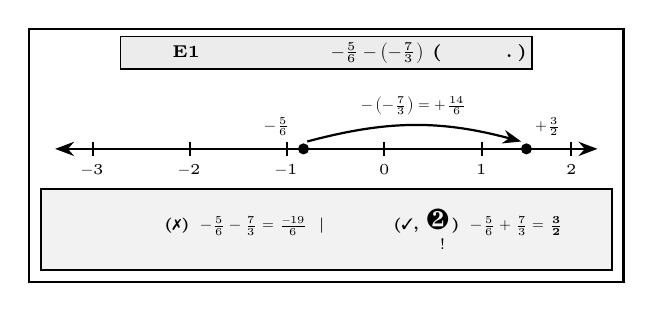
\begin{tikzpicture}[x=0.95cm, y=0.94cm, every node/.style={font=\scriptsize, text=black}]
  \draw[black, line width=0.95pt] (0,0) rectangle (7.95,3.42);
  \node[fill=gray!15, draw=black, line width=0.6pt, inner sep=2pt, font=\fontsize{6.2pt}{7.9pt}\selectfont\bfseries] at (3.975,3.10) {បេសកកម្ម \en{E1}៖ អន្ទាក់ដកចំនួនអវិជ្ជមាន $-\frac{5}{6} - \left(-\frac{7}{3}\right)$ (ឧទាហរណ៍ គ ទំ.៧)};

  % Number line from -3 to +2 (lowered to y=1.80 so arc clears top banner cleanly)
  \draw[black, line width=0.85pt, <->, >=Stealth] (0.35,1.80) -- (7.60,1.80);
  \foreach \x/\lbl in {0.85/-3, 2.15/-2, 3.45/-1, 4.75/0, 6.05/1, 7.25/2} {
    \draw[black, line width=0.7pt] (\x,1.71) -- (\x,1.89);
    \node[font=\fontsize{5.5pt}{6.9pt}\selectfont] at (\x,1.52) {$\lbl$};
  }
  \fill[black] (3.67,1.80) circle (2.0pt);
  \node[font=\fontsize{5.5pt}{7.0pt}\selectfont\bfseries] at (3.32,2.10) {$-\frac{5}{6}$};
  \fill[black] (6.65,1.80) circle (2.0pt);
  \node[font=\fontsize{5.5pt}{7.0pt}\selectfont\bfseries] at (6.94,2.10) {$+\frac{3}{2}$};
  \draw[black, line width=0.8pt, ->, >=Stealth] (3.72,1.90) to[bend left=15] node[above, font=\fontsize{5.4pt}{6.9pt}\selectfont] {$-\left(-\frac{7}{3}\right) = +\frac{14}{6}$} (6.58,1.90);

  % Bottom comparison box (2 clean lines inside box)
  \draw[black, line width=0.75pt, fill=gray!10] (0.16,0.16) rectangle (7.79,1.26);
  \node[align=center, font=\fontsize{5.5pt}{7.2pt}\selectfont] at (3.975,0.71) {\textbf{ច្រឡំលុបវង់ក្រចក (\ding{55})៖} $-\frac{5}{6}-\frac{7}{3}=\frac{-19}{6}$ \;\en{|}\; \textbf{សោត្រឹមត្រូវ (\ding{51}, \cnum{2})៖} $-\frac{5}{6}+\frac{7}{3}=\mathbf{\frac{3}{2}}$\\ការដកបំណុលអវិជ្ជមានចេញ ស្មើនឹង\textbf{ការបូកចំនួនផ្ទុយវិជ្ជមាន}!};
\end{tikzpicture}}

% ២. E2 POE 2: បន្ទះបំពេញឯកតាពេញ 1 (លំហាត់គំរូទី២ សិក្ខាសាលាសិល្បៈ ទំ.៨)
\newcommand{\figSeminarBarRATSUB}{%
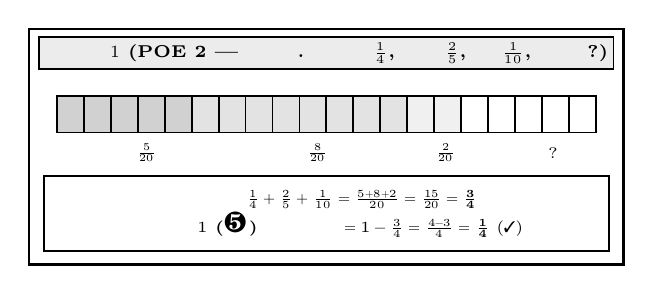
\begin{tikzpicture}[x=0.95cm, y=0.92cm, every node/.style={font=\scriptsize, text=black}]
  \draw[black, line width=0.95pt] (0,0) rectangle (7.95,3.25);
  \node[fill=gray!15, draw=black, line width=0.6pt, inner sep=2pt, font=\fontsize{6.2pt}{7.9pt}\selectfont\bfseries] at (3.975,2.92) {បន្ទះឯកតាពេញ $1$ (\en{POE 2} — គំរូទី២ ទំ.៨៖ តន្ត្រីករ $\frac{1}{4}$, សិល្បករ $\frac{2}{5}$, របាំ $\frac{1}{10}$, អ្នកនិពន្ធ?)};

  % 20-cell bar (width 0.36 each -> 20*0.36 = 7.20 from x=0.375 to 7.575)
  % 5 cells (1/4), 8 cells (2/5), 2 cells (1/10), 5 cells remaining (1/4)
  \foreach \i in {0,...,4}  { \fill[gray!36] (0.375+\i*0.36, 1.82) rectangle (0.375+\i*0.36+0.36, 2.32); }
  \foreach \i in {5,...,12} { \fill[gray!22] (0.375+\i*0.36, 1.82) rectangle (0.375+\i*0.36+0.36, 2.32); }
  \foreach \i in {13,14}    { \fill[gray!12] (0.375+\i*0.36, 1.82) rectangle (0.375+\i*0.36+0.36, 2.32); }
  \foreach \i in {0,...,19} { \draw[black, line width=0.65pt] (0.375+\i*0.36, 1.82) rectangle (0.375+\i*0.36+0.36, 2.32); }

  \node[font=\fontsize{5.4pt}{6.9pt}\selectfont] at (1.275,1.54) {តន្ត្រីករ $\frac{5}{20}$};
  \node[font=\fontsize{5.4pt}{6.9pt}\selectfont] at (3.615,1.54) {សិល្បករ $\frac{8}{20}$};
  \node[font=\fontsize{5.4pt}{6.9pt}\selectfont] at (5.415,1.54) {របាំ $\frac{2}{20}$};
  \node[font=\fontsize{5.5pt}{7.0pt}\selectfont\bfseries] at (6.675,1.54) {អ្នកនិពន្ធ $?$};

  \draw[black, line width=0.75pt] (0.20,0.18) rectangle (7.75,1.22);
  \node[align=center, font=\fontsize{5.6pt}{7.3pt}\selectfont] at (3.975,0.70) {បូកក្រុមទាំងបី៖ $\frac{1}{4}+\frac{2}{5}+\frac{1}{10} = \frac{5+8+2}{20} = \frac{15}{20} = \mathbf{\frac{3}{4}}$\\\textbf{ដកចេញពីឯកតាពេញ $1$ (\cnum{5})៖} ប្រភាគអ្នកនិពន្ធ $= 1 - \frac{3}{4} = \frac{4-3}{4} = \mathbf{\frac{1}{4}}$ (\ding{51})};
\end{tikzpicture}}

% ៣. E4 Contrast Box: -a - (-b) vs. -a - b
\newcommand{\figSignContrastRATSUB}{%
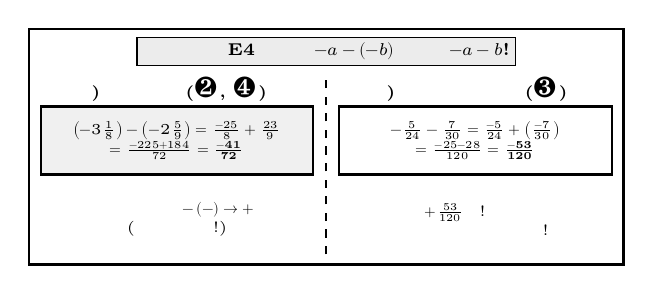
\begin{tikzpicture}[x=0.95cm, y=0.92cm, every node/.style={font=\scriptsize, text=black}]
  \draw[black, line width=0.95pt] (0,0) rectangle (7.95,3.25);
  \node[fill=gray!15, draw=black, line width=0.6pt, inner sep=2pt, font=\fontsize{6.2pt}{7.9pt}\selectfont\bfseries] at (3.975,2.94) {កាតប្រៀបធៀបសញ្ញា \en{E4}៖ កុំច្រឡំ $-a - (-b)$ ជាមួយនឹង $-a - b$!};

  \draw[black, dashed, line width=0.65pt] (3.975,0.14) -- (3.975,2.62);

  % Left: -a - (-b) (#9ខ p.12)
  \node[font=\fontsize{5.7pt}{7.3pt}\selectfont\bfseries] at (1.98,2.42) {១) ដកចំនួនអវិជ្ជមាន (\cnum{2}, \cnum{4})};
  \draw[black, line width=0.8pt, fill=gray!12] (0.16,1.24) rectangle (3.80,2.18);
  \node[align=center, font=\fontsize{5.5pt}{7.1pt}\selectfont] at (1.98,1.71) {$\left(-3\frac{1}{8}\right) - \left(-2\frac{5}{9}\right) = \frac{-25}{8} + \frac{23}{9}$\\$= \frac{-225 + 184}{72} = \mathbf{\frac{-41}{72}}$};
  \node[align=center, font=\fontsize{5.4pt}{6.9pt}\selectfont] at (1.98,0.62) {មានសញ្ញាដកជាប់គ្នា $-\,(-)\to\mathbf{+}$\\(ប្ដូរតួទី២ ទៅជាបូក!)};

  % Right: -a - b (ប្រតិបត្តិ ក p.8)
  \node[font=\fontsize{5.7pt}{7.3pt}\selectfont\bfseries] at (5.96,2.42) {២) ដកចំនួនវិជ្ជមានពីអវិជ្ជមាន (\cnum{3})};
  \draw[black, line width=0.8pt] (4.14,1.24) rectangle (7.79,2.18);
  \node[align=center, font=\fontsize{5.5pt}{7.1pt}\selectfont] at (5.965,1.71) {$-\frac{5}{24} - \frac{7}{30} = \frac{-5}{24} + \left(\frac{-7}{30}\right)$\\$= \frac{-25 - 28}{120} = \mathbf{\frac{-53}{120}}$};
  \node[align=center, font=\fontsize{5.4pt}{6.9pt}\selectfont] at (5.965,0.62) {\textbf{មិនមែន} $+\frac{53}{120}$ ទេ! ជំពាក់ថែមជំពាក់\\ត្រូវបូកតម្លៃដាច់ខាត រក្សាសញ្ញាដក!};
\end{tikzpicture}}

% ៤. E5 Diagnostic Cards A-D
\newcommand{\figExitCardsRATSUB}{%
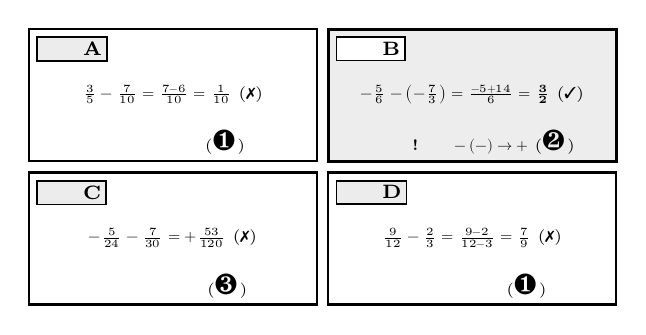
\begin{tikzpicture}[x=0.95cm, y=0.92cm, every node/.style={font=\scriptsize, text=black}]
  \draw[black, line width=0.9pt] (0,1.98) rectangle (3.85,3.80);
  \node[anchor=north west, fill=gray!15, draw=black, line width=0.6pt, inner sep=1.8pt] at (0.10,3.70) {\textbf{ជម្រើស \en{A}}};
  \node[font=\fontsize{5.7pt}{7.4pt}\selectfont] at (1.925,2.90) {$\frac{3}{5} - \frac{7}{10} = \frac{7-6}{10} = \frac{1}{10}$ (\ding{55})};
  \node[font=\fontsize{5.5pt}{7.1pt}\selectfont] at (1.925,2.24) {ច្រឡំត្រឡប់យកលេខធំដកតូច (\cnum{1})};

  \draw[black, line width=1.1pt, fill=gray!14] (4.00,1.98) rectangle (7.85,3.80);
  \node[anchor=north west, fill=white, draw=black, line width=0.6pt, inner sep=1.8pt] at (4.10,3.70) {\textbf{ជម្រើស \en{B}}};
  \node[font=\fontsize{5.7pt}{7.4pt}\selectfont] at (5.925,2.90) {$-\frac{5}{6} - \left(-\frac{7}{3}\right) = \frac{-5+14}{6} = \mathbf{\frac{3}{2}}$ (\ding{51})};
  \node[font=\fontsize{5.5pt}{7.1pt}\selectfont] at (5.925,2.24) {\textbf{ត្រឹមត្រូវ!} បើកសោ $-\,(-)\to +$ (\cnum{2})};

  \draw[black, line width=0.9pt] (0,0) rectangle (3.85,1.82);
  \node[anchor=north west, fill=gray!15, draw=black, line width=0.6pt, inner sep=1.8pt] at (0.10,1.72) {\textbf{ជម្រើស \en{C}}};
  \node[font=\fontsize{5.7pt}{7.4pt}\selectfont] at (1.925,0.92) {$-\frac{5}{24} - \frac{7}{30} = +\frac{53}{120}$ (\ding{55})};
  \node[font=\fontsize{5.5pt}{7.1pt}\selectfont] at (1.925,0.26) {ច្រឡំថាដកពីរដងក្លាយជាបូក (\cnum{3})};

  \draw[black, line width=0.9pt] (4.00,0) rectangle (7.85,1.82);
  \node[anchor=north west, fill=gray!15, draw=black, line width=0.6pt, inner sep=1.8pt] at (4.10,1.72) {\textbf{ជម្រើស \en{D}}};
  \node[font=\fontsize{5.7pt}{7.4pt}\selectfont] at (5.925,0.92) {$\frac{9}{12} - \frac{2}{3} = \frac{9-2}{12-3} = \frac{7}{9}$ (\ding{55})};
  \node[font=\fontsize{5.5pt}{7.1pt}\selectfont] at (5.925,0.26) {អន្ទាក់ដកភាគបែងនឹងភាគបែង (\cnum{1})};
\end{tikzpicture}}

\begin{document}
\fontsize{10pt}{15.2pt}\selectfont

% -------------------- ក្បាលកិច្ចតែងការ --------------------
\begin{center}
  {\muol\fontsize{11pt}{16pt}\selectfont ព្រះរាជាណាចក្រកម្ពុជា}\\[2pt]
  {\muol\fontsize{10pt}{15pt}\selectfont ជាតិ សាសនា ព្រះមហាក្សត្រ}\\[1pt]
  \khmflourish
\end{center}

\vspace{-24pt}
{\muol\fontsize{9.5pt}{12.5pt}\selectfont
មន្ទីរអប់រំ យុវជន និងកីឡា ខេត្តកំពង់ធំ\\
ការិយាល័យអប់រំ យុវជន និងកីឡា ស្រុកកំពង់ស្វាយ\\
អនុវិទ្យាល័យព្រះក្រសាំង}

\vspace{1pt}
\begin{center}
  {\muol\fontsize{10pt}{14pt}\selectfont កិច្ចតែងការបង្រៀន}
\end{center}
\vspace{0pt}

% -------------------- ព័ត៌មានទូទៅ --------------------
{\renewcommand{\arraystretch}{0.98}
\hspace*{3.1cm}%
\begin{tabular}{@{}l l L{11.0cm}@{}}
  - \hspace{0.35cm} មុខវិជ្ជា & : & គណិតវិទ្យា ថ្នាក់ទី៨ (ពីជគណិត) \\
  - \hspace{0.35cm} ចំណងជើងមេរៀន & : & មេរៀនទី១៖ ចំនួនសនិទាន \\
  - \hspace{0.35cm} ចំណងជើងរង & : & ៣.៣. ប្រមាណវិធីដកនៃចំនួនសនិទាន (ទំ.៧–៨) \\
  - \hspace{0.35cm} រយៈពេល & : & ១ ម៉ោងសិក្សា (៥០ នាទី) \\
  - \hspace{0.35cm} បង្រៀនដោយ & : & ហុក ប៊ុនថែន \\
  - \hspace{0.35cm} កាលបរិច្ឆេទ & : & ថ្ងៃព្រហស្បតិ៍ ទី១៩ ខែវិច្ឆិកា ឆ្នាំ២០២៦ \\
\end{tabular}

\vspace{2pt}

% -------------------- I. វត្ថុបំណង --------------------
\textbf{I.} {\muol វត្ថុបំណង}\\[1pt]
\hspace*{0.55cm}%
\begin{tabular}{@{}l l L{14.2cm}@{}}
  \wcirc \hspace{0.25cm} វិជ្ជាសម្បទា & : & សិស្សប្រាប់រូបមន្តដកចំនួនសនិទាន ($\frac{a}{b}-\frac{c}{b}=\frac{a-c}{b}$, $\frac{a}{b}-\frac{c}{d}=\frac{ad-bc}{bd}$) និងបកស្រាយវិធីដកជាការបូកនឹងចំនួនផ្ទុយ ($\frac{a}{b}-\frac{c}{d}=\frac{a}{b}+\left(-\frac{c}{d}\right)$) បានត្រឹមត្រូវតាមសៀវភៅគោល (ទំ.៧–៨) ។ \\
  \wcirc \hspace{0.25cm} បំណិនសម្បទា & : & សិស្សគណនាផលដកប្រភាគមានសញ្ញា ចំនួនចម្រុះ និងដោះស្រាយចំណោទរកប្រភាគនៅសល់ពីឯកតាពេញ $1$ ដោយដៃលើសន្លឹកកិច្ចការបានត្រឹមត្រូវ ។ \\
  \wcirc \hspace{0.25cm} ចរិយាសម្បទា & : & សិស្សមានទម្លាប់គូសរង្វង់ពិនិត្យសញ្ញាដកជាប់វង់ក្រចកដោយប្រុងប្រយ័ត្ន ជៀសវាងកំហុសច្រឡំសញ្ញាក្នុងការគណនាទិន្នន័យជាក់ស្ដែង ។ \\
\end{tabular}

\vspace{2pt}

% -------------------- II. សម្ភារៈឧបទេស --------------------
\textbf{II.} {\muol សម្ភារៈឧបទេស}\\[1pt]
\hspace*{0.55cm}$\bullet$ \hspace{0.35cm} សៀវភៅសិក្សាគោលគណិតវិទ្យាថ្នាក់ទី៨ (ទំ.៧–៨ និងទំ.១២) ក្ដារខៀន ដីស និងសន្លឹកកិច្ចការសិស្ស ស-ខ្មៅ (\en{Worksheet\_RAT\_SUB} ទំព័រ ១–២ គ្មានស្លាយ \en{LCD} គ្មានម៉ាស៊ីនគិតលេខ)

\vspace{2pt}

% -------------------- III. វិធីសាស្រ្តបង្រៀន --------------------
\textbf{III.} {\muol វិធីសាស្រ្តបង្រៀន}\\[1pt]
\hspace*{0.45cm}%
\begin{tabular}{@{}l l L{14.85cm}@{}}
  $\bullet$ \hspace{0.25cm} គោលវិធី & : & សិស្សមជ្ឈមណ្ឌល (បង្រៀនតាមសន្លឹកកិច្ចការស៊ើបអង្កេតជាដៃគូ និងក្ដារខៀន គ្មាន \en{LCD}) \\
  $\bullet$ \hspace{0.25cm} យុទ្ធវិធីបង្រៀន & : & គំរូ \en{5Es} រួមបញ្ចូលបន្ទាត់ចំនួនទិសដៅ-សោសញ្ញាដកពីរជាន់ \en{(POE 1)} និងបន្ទះបំពេញឯកតាពេញ $1$ \en{(POE 2)} \\
\end{tabular}
}

\vspace{2pt}

% -------------------- IV. ដំណើរការបង្រៀន --------------------
\textbf{IV.} {\muol ដំណើរការបង្រៀន}

\vspace{1pt}

\renewcommand{\arraystretch}{1.15}
\begin{longtable}{|L{5.50cm}|L{7.90cm}|L{4.80cm}|}
\hline
\rowcolor{headgray}
\multicolumn{1}{|c|}{\muol សកម្មភាពគ្រូ} &
\multicolumn{1}{c|}{\muol ខ្លឹមសារមេរៀន} &
\multicolumn{1}{c|}{\muol សកម្មភាពសិស្ស} \\
\hline
\endfirsthead

\hline
\rowcolor{headgray}
\multicolumn{1}{|c|}{\muol សកម្មភាពគ្រូ} &
\multicolumn{1}{c|}{\muol ខ្លឹមសារមេរៀន} &
\multicolumn{1}{c|}{\muol សកម្មភាពសិស្ស} \\
\hline
\endhead

\hline
\endfoot

\hline
\endlastfoot

% ==================== ជំហានទី១ (2min) ====================
\stepheader{ជំហានទី១ \enbf{(}រដ្ឋបាលថ្នាក់\enbf{)}}
$\bullet$ ពិនិត្យអវត្តមាន អនាម័យ និងសណ្ដាប់ធ្នាប់ថ្នាក់រៀន \timenote{(2 min)}\par\vspace{2pt}
$\bullet$ ចែក \textbf{សន្លឹកកិច្ចការសិស្ស (\en{Worksheet\_RAT\_SUB})} ម្នាក់ ១ សន្លឹក (ផ្កាប់ទុកសិន)
&
$\bullet$ រដ្ឋបាលថ្នាក់ និងការរៀបចំដៃគូសិក្សា (២ នាក់ក្នុង ១ តុ)\par\vspace{2pt}
$\bullet$ សន្លឹកកិច្ចការសិស្ស ស-ខ្មៅ ២ ទំព័រ សម្រាប់បំពេញតាមជំហានមេរៀន
&
$\circ$ ប្រធានថ្នាក់រាយការណ៍អវត្តមាន\par\vspace{2pt}
$\circ$ ទទួលសន្លឹកកិច្ចការ ដាក់ផ្កាប់លើតុ \\[3pt]
\hline

% ==================== ជំហានទី២ (9min: <=3 + 3 + E1 3) ====================
\stepheader{ជំហានទី២ \enbf{(}កិច្ចការផ្ទះ \enbf{+} ទំនាក់ទំនងមេរៀនថ្មី\enbf{)}}
\timenote{កំណែកិច្ចការផ្ទះ ($\le 3\unit{min}$)}\par\vspace{2pt}
$\bullet$ ហៅសិស្ស ២ នាក់ឡើងកែកិច្ចការផ្ទះចំណុច ៣.១–៣.២ លើក្ដារខៀន
&
\textbf{១. កំណែកិច្ចការផ្ទះ (ប្រមាណវិធីបូក និងលក្ខណៈផ្គុំ)៖}\par\vspace{2pt}
$\bullet$ \textbf{១ក)} $\left(-\dfrac{1}{8}\right)+\left(2\dfrac{5}{9}\right) = \dfrac{-9+184}{72} = \dfrac{175}{72}$ \;;\; \textbf{១គ)} $-1\dfrac{3}{4}+\dfrac{5}{-6}+\dfrac{7}{12} = -2$\par\vspace{2pt}
$\bullet$ \textbf{២)} $\left(\dfrac{-3}{11}+\dfrac{5}{12}\right)+\left(\dfrac{7}{12}+\dfrac{3}{11}\right) = 0 + \dfrac{12}{12} = 1$
&
$\circ$ តំណាងសិស្សឡើងកែលើក្ដារខៀន\par\vspace{2pt}
$\circ$ ផ្ទៀងផ្ទាត់ និងកែតម្រូវចូលសៀវភៅ \\[3pt]

\timenote{រំលឹកមេរៀនទាក់ទង (3 min)}\par\vspace{2pt}
$\bullet$ សួររំលឹកចំនួនផ្ទុយនៃប្រភាគអវិជ្ជមាន៖ «តើ $-\left(-\frac{7}{3}\right)$ ស្មើប៉ុន្មាន?»
&
\textbf{២. រំលឹកចំនួនផ្ទុយ និងការដកចំនួនគត់រ៉ឺឡាទីប៖}\par\vspace{2pt}
$\bullet$ ចំនួនផ្ទុយ៖ $-\left(-\dfrac{7}{3}\right) = +\dfrac{7}{3}$ \;;\; ក្បួនដកចំនួនគត់៖ $a - b = a + (-b)$
&
$\circ$ ឆ្លើយផ្ទាល់មាត់៖ ចំនួនផ្ទុយគឺ $+\frac{7}{3}$ \\[3pt]

$\bullet$ សួរបន្តពីការដកចំនួនគត់រ៉ឺឡាទីប៖ «តើ $(-5) - (-14)$ និង $6 - 7$ ស្មើប៉ុន្មាន?»
&
$\bullet$ អនុវត្តចំនួនគត់៖ $(-5) - (-14) = -5 + 14 = +9$ \;;\; $6 - 7 = -1$
&
$\circ$ ឆ្លើយផ្ទាល់មាត់៖ $+9$ និង $-1$ \\[3pt]

\fiveE{E1 - Engage} \timenote{(3 min)}\par\vspace{2pt}
$\bullet$ ឱ្យសិស្សផ្ងារសន្លឹកកិច្ចការទំព័រទី១ អានបេសកកម្ម \en{E1} (ឧទាហរណ៍ គ ទំ.៧)៖ «គណនាផលដក $-\frac{5}{6} - \left(-\frac{7}{3}\right)$ ។ សិស្សម្នាក់សរសេរ $-\frac{5}{6} - \frac{7}{3} = \frac{-19}{6}$»\par\vspace{2pt}
\hspace*{0.3em}-- សំណួរបំផុស៖ «បើដកបំណុលអវិជ្ជមាន $-\frac{7}{3}$ ចេញ តើតម្លៃកើនឡើងទៅស្ដាំ ឬថយចុះទៅឆ្វេងលើបន្ទាត់ចំនួន?»
&
\textbf{៣. បេសកកម្ម \en{E1} — អន្ទាក់ដកចំនួនអវិជ្ជមាន៖}\par\vspace{2pt}
$\bullet$ ការលុបវង់ក្រចក $-\,\left(-\frac{7}{3}\right)$ ទៅជា $-\frac{7}{3}$ ធ្វើឱ្យទិសដៅដើរបញ្ច្រាស!\par\vspace{2pt}
$\bullet$ ភ្ជាប់ចូលមេរៀនថ្មី៖ \textbf{៣.៣. ប្រមាណវិធីដកនៃចំនួនសនិទាន (ទំ.៧–៨)}
&
$\circ$ គូសធីកការទស្សន៍ទាយលើសន្លឹកកិច្ចការ និងពិភាក្សាទិសដៅលើបន្ទាត់ចំនួន \\[3pt]

& \cfig{\figEngageRATSUB} & \\[3pt]
\hline

% ==================== ជំហានទី៣ (17min: E2 11 + E3 6) ====================
\stepheader{ជំហានទី៣ \enbf{(}ខ្លឹមសារមេរៀនថ្មី\enbf{)}}
\fiveE{E2 - Explore} \timenote{(11 min)}\par\vspace{2pt}
$\bullet$ សរសេរចំណងជើងមេរៀនលើក្ដារខៀន និងណែនាំ \textbf{សកម្មភាពទី១ (\en{POE 1})} លើសន្លឹកកិច្ចការ (ឧទាហរណ៍ ក, ខ និងគំរូទី១ ក ទំ.៧)
&
\textbf{៣.៣. ប្រមាណវិធីដកនៃចំនួនសនិទាន (ទំ.៧–៨) — \en{POE 1}៖}\par\vspace{2pt}
$\bullet$ \textbf{ឧទាហរណ៍ ក, ខ (ទំ.៧)៖} $\dfrac{9}{10}-\dfrac{7}{10}=\dfrac{2}{10}=\dfrac{1}{5}$ \;;\; $\dfrac{5}{4}-\dfrac{7}{8}=\dfrac{10-7}{8}=\dfrac{3}{8}$
&
$\circ$ កត់ចំណងជើងមេរៀន និងបំពេញផលដកប្រភាគក្នុងតារាង \en{POE 1} \\[3pt]

$\bullet$ ឱ្យដៃគូប្រៀបធៀបករណីតួទី១ តូចជាងតួទី២ (គំរូទី១ ក) និងករណីសោសញ្ញាដកពីរជាន់ (ឧទាហរណ៍ គ ទំ.៧)
&
$\bullet$ \textbf{គំរូទី១ ក (ទំ.៧)៖} $\dfrac{3}{5}-\dfrac{7}{10} = \dfrac{6-7}{10} = \graybox{$\dfrac{-1}{10}$} \neq \dfrac{1}{10}$ (ហាមត្រឡប់ $7-6$!)\par\vspace{2pt}
$\bullet$ \textbf{ឧទាហរណ៍ គ (ទំ.៧)៖} $-\dfrac{5}{6}-\left(-\dfrac{7}{3}\right) = \dfrac{-5}{6}+\dfrac{7}{3} = \dfrac{-5+14}{6} = \dfrac{9}{6} = \graybox{$\dfrac{3}{2}$}$
&
$\circ$ គូសរង្វង់សោសញ្ញា \textbf{[$-(-)\to +$]} និងរកឃើញថាផលដកស្មើ $+\frac{3}{2}$ \\[3pt]

$\bullet$ ណែនាំ \textbf{សកម្មភាពទី២ (\en{POE 2} — បន្ទះបំពេញឯកតាពេញ $1$)} តាម \textbf{លំហាត់គំរូទី២} (សិក្ខាសាលាសិល្បៈ ទំ.៨)៖\par\vspace{2pt}
\hspace*{0.3em}-- \textbf{ទស្សន៍ទាយ (\en{P})៖} «បើតន្ត្រីករ $\frac{1}{4}$, សិល្បករ $\frac{2}{5}$ និងអ្នករបាំ $\frac{1}{10}$ តើប្រភាគអ្នកនិពន្ធនៅសល់ស្មើប៉ុន្មាននៃអ្នកចូលរួមទាំងអស់ ($1$)?»
&
\textbf{លំហាត់គំរូទី២ (ទំ.៨ — បន្ទះឯកតាពេញ $1$) — \en{POE 2}៖}\par\vspace{2pt}
$\bullet$ ប្រភាគតន្ត្រីករ សិល្បករ និងអ្នករបាំ៖ $\dfrac{1}{4}+\dfrac{2}{5}+\dfrac{1}{10} = \dfrac{5+8+2}{20} = \dfrac{15}{20} = \dfrac{3}{4}$\par\vspace{2pt}
$\bullet$ ប្រភាគអ្នកនិពន្ធនៅសល់៖ $1 - \dfrac{3}{4} = \dfrac{4-3}{4} = \graybox{$\dfrac{1}{4}$}$
&
$\circ$ រាប់ក្រឡា $15$ ក្នុង $20$ ក្រឡាលើសន្លឹកកិច្ចការ រួចដកចេញពីឯកតាពេញ $1$ ឃើញនៅសល់ $\frac{1}{4}$ \\[3pt]

& \cfig{\figSeminarBarRATSUB} & \\[3pt]

\fiveE{E3 - Explain} \timenote{(6 min)}\par\vspace{2pt}
$\bullet$ ហៅតំណាងដៃគូឡើងបង្គុំរូបមន្តទូទៅនៃប្រមាណវិធីដក (ទំ.៧) លើក្ដារខៀន
&
\textbf{សំយោគបញ្ញត្តិ និងធនាគារហេតុផល \en{B\&W} (\cnum{1}--\cnum{5})៖}\par\vspace{2pt}
$\bullet$ \textbf{ជាទូទៅ (ទំ.៧)៖} $\dfrac{a}{b}-\dfrac{c}{d} = \dfrac{ad-bc}{bd}$ \;;\; \textbf{សម្គាល់៖} $\dfrac{a}{b}-\dfrac{c}{b} = \dfrac{a-c}{b}$
&
$\circ$ កត់ត្រារូបមន្តប្រអប់ «ជាទូទៅ» លើសន្លឹកកិច្ចការ \\[3pt]

$\bullet$ បញ្ជាក់ទំនាក់ទំនងប្ដូរដកជាបូកចំនួនផ្ទុយ និងបង្ហាញថាវិធីដកគ្មានលក្ខណៈត្រឡប់ទេ
&
$\bullet$ \textbf{ប្ដូរដកជាបូកចំនួនផ្ទុយ៖} $\dfrac{a}{b}-\dfrac{c}{d} = \dfrac{a}{b}+\left(-\dfrac{c}{d}\right)$ \;;\; $\dfrac{a}{b}-\dfrac{c}{d} \neq \dfrac{c}{d}-\dfrac{a}{b}$
&
$\circ$ បំពេញប្រអប់រូបមន្តផ្នែកទី២ លើសន្លឹកកិច្ចការ \\[3pt]

$\bullet$ កត់ធនាគារហេតុផល \cnum{1}--\cnum{3} លើក្ដារខៀន សម្រាប់យោងពេលដោះស្រាយលំហាត់
&
\cnum{1} តម្រូវភាគបែងរួមសិន ទើបយកភាគយកទី១ ដកភាគយកទី២ (ហាមត្រឡប់!) ។\par\vspace{1.5pt}
\cnum{2} សោសញ្ញាដកពីរជាន់៖ $a - (-b) = a + b$ (ដកចំនួនអវិជ្ជមាន ស្មើបូកចំនួនវិជ្ជមាន) ។\par\vspace{1.5pt}
\cnum{3} ដកថែមពីចំនួនអវិជ្ជមាន៖ $-a - b = -a + (-b) = -(a+b)$ (រក្សាសញ្ញាដក) ។
&
$\circ$ ផ្ទៀងផ្ទាត់ហេតុផល \cnum{1}--\cnum{3} លើសន្លឹកកិច្ចការ \\[3pt]

$\bullet$ បញ្ជាក់ហេតុផល \cnum{4}--\cnum{5} សម្រាប់ចំនួនចម្រុះ និងចំណោទឯកតាពេញ $1$
&
\cnum{4} ចំនួនចម្រុះអវិជ្ជមាន៖ $-k\frac{r}{b} = -\frac{kb+r}{b}$ មុននឹងបើកសោសញ្ញា ។\par\vspace{1.5pt}
\cnum{5} រកប្រភាគនៅសល់ពីទាំងមូល៖ យក $1 = \frac{b}{b}$ ដកផលបូកប្រភាគផ្នែកដែលស្គាល់ ។
&
$\circ$ ធ្វើលំហាត់ត្រួតពិនិត្យរហ័សនៅបាតទំព័រទី១ \\[3pt]
\hline

% ==================== ជំហានទី៤ (20min: E4 10 + E5 10) ====================
\stepheader{ជំហានទី៤ \enbf{(}ពង្រឹង និងពង្រីកចំណេះដឹង\enbf{)}}
\fiveE{E4 - Elaborate} \timenote{(10 min)}\par\vspace{2pt}
$\bullet$ ឱ្យសិស្សបើកសន្លឹកកិច្ចការទំព័រទី២ (ផ្នែកទី៣) គណនា \textbf{លំហាត់គំរូទី១ ខ} (ទំ.៧) និង \textbf{លំហាត់ \#9ខ} (ទំ.១២)
&
\textbf{១. លំហាត់ពង្រីកចំណេះដឹង (ទំ.៧ និងទំ.១២ \#9ខ, \#10ង)៖}\par\vspace{2pt}
$\bullet$ \textbf{ក) គំរូទី១ ខ (ទំ.៧)៖} $\dfrac{9}{12}-\dfrac{2}{3} = \dfrac{9-8}{12} = \graybox{$\dfrac{1}{12}$} \quad (\text{\cnum{1}})$\par\vspace{2pt}
$\bullet$ \textbf{ខ) ទំ.១២ \#9ខ៖} $\left(-3\dfrac{1}{8}\right)-\left(-2\dfrac{5}{9}\right) = \dfrac{-25}{8}+\dfrac{23}{9} = \dfrac{-225+184}{72} = \graybox{$\dfrac{-41}{72}$}$
&
$\circ$ បំពេញជំហានបំប្លែងចំនួនចម្រុះ និងបើកសោសញ្ញាក្នុងតារាង \en{E4} \\[3pt]

$\bullet$ ណែនាំកន្សោមចម្រុះបូក-ដកបីតួ (ទំ.១២ \#10ង) និងសំណួរឆ្លុះបញ្ចាំង \en{EIA Looking-Back}
&
$\bullet$ \textbf{គ) ទំ.១២ \#10ង៖} $-\dfrac{11}{8}+\dfrac{21}{4}-\dfrac{17}{16} = \dfrac{-22+84-17}{16} = \graybox{$\dfrac{45}{16}$}$\par\vspace{2pt}
$\bullet$ \textbf{ឆ្លុះបញ្ចាំង៖} ញែកឱ្យដាច់រវាង $-a-(-b)=-a+b$ និង $-a-b=-(a+b)$!
&
$\circ$ ពិភាក្សាឆ្លើយសំណួរ \en{EIA Looking-Back} ប្រៀបធៀបសញ្ញាទាំងពីរករណី \\[3pt]

& \cfig{\figSignContrastRATSUB} & \\[3pt]

\fiveE{E5 - Evaluate} \timenote{(10 min)}\par\vspace{2pt}
$\bullet$ ឱ្យសិស្សធ្វើលំហាត់ \textbf{ប្រតិបត្តិ} (ទំ.៨ ក និង ខ) លើសន្លឹកកិច្ចការ រួចប្ដូរសន្លឹកផ្ទៀងផ្ទាត់ (\en{Pause-Review})
&
\textbf{២. ប្រតិបត្តិ (ទំ.៨) និងចម្លើយបិទបេសកកម្ម \en{E1}៖}\par\vspace{2pt}
$\bullet$ \textbf{ក)} $-\dfrac{5}{24}-\dfrac{7}{30} = \dfrac{-25-28}{120} = \graybox{$\dfrac{-53}{120}$} \quad (\text{PPCM}(24,30)=120,\; \text{\cnum{3}})$\par\vspace{2pt}
$\bullet$ \textbf{ខ)} $\dfrac{1}{15}-\dfrac{27}{50} = \dfrac{10-81}{150} = \graybox{$\dfrac{-71}{150}$} \quad (\text{PPCM}(15,50)=150,\; \text{\cnum{1}})$
&
$\circ$ គណនាប្រតិបត្តិទំ.៨ ដោយដៃ និងផ្ទៀងផ្ទាត់សញ្ញាជាដៃគូ \\[3pt]

$\bullet$ ហៅតំណាងដៃគូឆ្លើយបិទបញ្ចប់បេសកកម្ម \en{E1} លើក្ដារខៀន
&
$\bullet$ \textbf{បិទ \en{E1}៖} $-\dfrac{5}{6}-\left(-\dfrac{7}{3}\right) = \dfrac{-5}{6}+\dfrac{14}{6} = \dfrac{9}{6} = \mathbf{+\dfrac{3}{2}}$ \mbox{(\cnum{2})!}
&
$\circ$ តំណាងដៃគូបកស្រាយការបើកសោសញ្ញាបិទបញ្ចប់ \en{E1} \\[3pt]

$\bullet$ វាយតម្លៃរហ័ស \textbf{៦០ វិនាទី}៖ ឱ្យសិស្សគូសវង់ជម្រើសត្រឹមត្រូវក្នុងប្រអប់ \en{A--D} និងបំពេញសំបុត្រចេញ
&
\textbf{៣. វិនិច្ឆ័យកំហុសរហ័ស (\en{A--D})៖} ចម្លើយត្រឹមត្រូវគឺ \graybox{\textbf{ជម្រើស \en{B}}} ($\frac{3}{2}$) ។\par\vspace{2pt}
(\en{A} ច្រឡំត្រឡប់ $7-6$; \en{C} ច្រឡំថាដកពីរដងក្លាយជាបូក; \en{D} ដកភាគបែងខុសក្បួន)
&
$\circ$ គូសវង់ជម្រើស \en{B} និងបំពេញសំបុត្រចេញមុនបញ្ចប់ម៉ោង \\[3pt]

& \cfig{\figExitCardsRATSUB} & \\[3pt]
\hline

% ==================== ជំហានទី៥ (<=2min) ====================
\stepheader{ជំហានទី៥ \enbf{(}កិច្ចការផ្ទះ \enbf{+} បណ្ដាំផ្ញើ\enbf{)}}
\timenote{ចំណាយពេលឱ្យតិចបំផុតកុំឱ្យលើស 2 min}\par\vspace{2pt}
$\bullet$ ណែនាំកិច្ចការផ្ទះនៅផ្នែកទី៥ នៃសន្លឹកកិច្ចការ និងផ្ដាំផ្ញើឱ្យអានមុនចំណុច \textbf{៤. ប្រមាណវិធីគុណនៃចំនួនសនិទាន} (ទំ.៨–៩)
&
\centerline{\muol កិច្ចការផ្ទះ}\par\vspace{2pt}
$\bullet$ \textbf{លំហាត់ ១៖} គណនា រួចសម្រួល៖ ក) $\dfrac{7}{12}-\dfrac{5}{8}$ \quad ខ) $-\dfrac{3}{14}-\left(-\dfrac{5}{21}\right)$ \quad គ) $\left(-2\dfrac{1}{5}\right)-\left(-\dfrac{7}{9}\right)$\par\vspace{2pt}
$\bullet$ \textbf{លំហាត់ ២៖} គ្រួសារមួយចំណាយប្រាក់ចំណូលលើម្ហូប $\frac{1}{2}$ និងទឹក-ភ្លើង $\frac{1}{10}$ ។ រកប្រភាគប្រាក់នៅសល់ ។\par\vspace{2pt}
$\bullet$ \textbf{បណ្ដាំផ្ញើ៖} អានមុនចំណុច \textbf{៤. ប្រមាណវិធីគុណនៃចំនួនសនិទាន} (សៀវភៅពុម្ព ទំ.៨–៩) ។
&
$\circ$ កត់ត្រាកិច្ចការផ្ទះ និងទទួលបណ្ដាំផ្ញើដោយសណ្ដាប់ធ្នាប់ \\[3pt]
\end{longtable}

% -------------------- កាលបរិច្ឆេទ និងហត្ថលេខា --------------------
\vspace{2pt}
\hfill
\begin{minipage}{9.8cm}
  {\centering
    ថ្ងៃព្រហស្បតិ៍ ១០កើត ខែកត្តិក ឆ្នាំមមី អដ្ឋស័ក ពុទ្ធសករាជ ២៥៧០\\[2pt]
    ត្រូវនឹងថ្ងៃទី១៩ ខែវិច្ឆិកា ឆ្នាំ២០២៦\\[3pt]
    {\muol គ្រូបង្រៀន}\par}
  \vspace{28pt}
  \hfill{\muol ហុក ប៊ុនថែន}\hspace*{1.4cm}
\end{minipage}

\end{document}
